\section{Study 2 --- Capability Gap Analysis}
\label{sec:method-study2}

This study measures how much of the enterprise's current platform a European
provider could replace. It works from a fixed list of sixty \acs{AWS} services
and asks of every provider whether it offers an equivalent, so what follows
describes where that list came from and how the answers were scored.

The instrument has two parts: a catalogue of services grouped into eleven
categories, and two further dimensions assessed directly rather than from the
catalogue.

\subsection*{The reference catalogue}

The list is drawn from the \acs{AWS} product catalogue
\cite{AWS_Products}, narrowed to what the enterprise uses. Fifty of the sixty
services come from a checklist completed by Alps Alpine
\cite{AlpsAlpine_Checklist}, which asked, for each capability, whether it
was necessary previously, now or later, and named the \acs{AWS} service that
provides it. Fifty-eight lines were marked as needed; several name the same
product, leaving fifty distinct services. A further ten in common use elsewhere
were added, so that a provider is not credited with completeness merely because
the enterprise does not currently need a category.

\todo{The sources for the ten added services.}

The checklist was completed against the platform shown in
\cref{fig:alps-infrastructure} in \cref{app:checklist}, which maps the services the department runs, is
investigating, or expects to need. It is arranged in six stages, from the
networking and identity foundation on the left through to the applications users
see on the right, and it shows why the catalogue is weighted as it is: security
and identity carry the largest number of distinct services, and the specialised
categories --- machine learning and device management --- sit furthest from the
foundation.

\acs{AWS} is the baseline. Every one of the sixty services is its own, so it
scores full marks on every dimension by construction, and each European provider
is measured by how much of the catalogue it matches. The consequence noted in
\cref{sec:research-design} follows from this: a provider offering something
\acs{AWS} does not offer earns nothing for it.

\subsection*{The thirteen dimensions}

The eleven categories are scored from the services they contain. Two further
dimensions --- scalability and performance --- cannot be settled by counting
services, and were assessed instead from what each provider publishes about its
regions, its scaling, its largest instances, its service-level commitments and
its certifications. \Cref{tab:readiness-dimensions} lists all thirteen.

\begin{table}[htbp]
  \centering
  \caption{The thirteen readiness dimensions. Eleven are scored from the
           services they contain; scalability and performance are assessed from
           published documentation.}
  \label{tab:readiness-dimensions}
  \small
  \begin{tabularx}{\textwidth}{@{}l r X@{}}
    \toprule
    \textbf{Dimension} & \textbf{Services} & \textbf{What it covers} \\
    \midrule
    Scalability  & --- & Regions and zones, auto-scaling, largest instance available \\
    Performance  & --- & Published service-level commitments, certifications, storage and network specification \\
    \midrule
    Web and App Hosting &  1 & Managed web and application hosting \\
    Compute      &  6 & Virtual machines, containers, serverless functions, batch \\
    Storage      &  5 & Object, block, archival, backup and shared file storage \\
    Database     &  7 & Relational, document, key-value, time-series, cache, warehouse \\
    Networking   &  7 & Load balancing, private networking, \acs{DNS}, \acs{API} gateway, \acs{CDN}, dedicated links \\
    AI/ML        &  6 & Image recognition, model training, language models, \acs{ETL}, analytics \\
    Security     & 12 & Identity, keys, secrets, certificates, threat detection, firewall, audit logging \\
    Monitoring   &  4 & Metrics, logs, alerting, incident management, cost reporting \\
    Dev/Deploy   &  5 & Build, deployment, pipelines, container registry, infrastructure as code \\
    IoT          &  2 & Device connectivity and fleet management \\
    Messaging    &  5 & Queues, event bus, workflow orchestration, email, streaming \\
    \midrule
    & \textbf{60} & \\
    \bottomrule
  \end{tabularx}
\end{table}

The categories are of very unequal size, which matters when reading a dimension
score. Web and app hosting contains one service, so a provider either scores nothing
there or scores full marks; security contains twelve, so a single service moves
it by four points. The dimensions are therefore comparable as proportions of what
each contains, not as equally fine measurements.

\subsection*{The sixty services}

\Cref{tab:readiness-services} gives the catalogue, grouped by dimension. Services
shown without a mark are those Alps Alpine Europe uses or expects to need; the
ten marked with a dagger are widely used elsewhere and were added so that a
provider is not credited with completeness merely because the department does not
currently need a category.

\begin{table}[htbp]
\centering
\caption{The sixty reference services, by dimension. Unmarked services are used
  by Alps Alpine Europe \cite{AlpsAlpine_Checklist};
  \quad{\normalfont($^{\dagger}$ = popular elsewhere in the industry, added for
  completeness)}}
\label{tab:readiness-services}
\resizebox{\linewidth}{!}{%
\renewcommand{\arraystretch}{1.15}
\begin{tabularx}{1.62\linewidth}{XXXXXXX}
\toprule
\textbf{Scalability}        & \textbf{Performance}       & \textbf{Web and App Hosting (1)} &
\textbf{Compute (6)}        & \textbf{Storage (5)}       & \textbf{Database (7)}    &
\textbf{Networking (7)} \\
\midrule
\textit{Assessed}           & \textit{Assessed}          & Amplify                  &
Lambda                      & S3                         & RDS                      &
App.\ Load Balancer \\
\textit{directly}           & \textit{directly}          &                          &
ECS                         & S3 Glacier                 & DocumentDB               &
Net.\ Load Balancer \\
                            &                            &                          &
EKS                         & EBS                        & DynamoDB                 &
VPC \\
                            &                            &                          &
EC2                         & Backup                     & Timestream               &
Route~53 \\
                            &                            &                          &
Batch                       & EFS$^{\dagger}$            & Aurora$^{\dagger}$       &
API Gateway \\
                            &                            &                          &
Elastic Beanstalk$^{\dagger}$ &                          & ElastiCache$^{\dagger}$  &
CloudFront$^{\dagger}$ \\
                            &                            &                          &
                            &                            & Redshift$^{\dagger}$     &
Direct Connect$^{\dagger}$ \\
\midrule
\textbf{AI/ML (6)}          & \textbf{Security (12)}     & \textbf{Monitoring (4)}  &
\textbf{Dev/Deploy (5)}     & \textbf{IoT (2)}           & \textbf{Messaging (5)}   &
\\
\midrule
Rekognition                 & IAM                        & CloudWatch               &
CodeBuild                   & IoT Core                   & SQS                      & \\
SageMaker                   & Cognito                    & SNS                      &
CodeDeploy                  & IoT Device Mgmt.           & EventBridge              & \\
Bedrock                     & IAM Identity Center        & Systems Manager          &
CodePipeline                &                            & Step Functions           & \\
Glue                        & KMS                        & Cost Explorer            &
ECR                         &                            & SES                      & \\
EMR                         & Secrets Manager            &                          &
CloudFormation$^{\dagger}$  &                            & Kinesis$^{\dagger}$      & \\
Athena                      & Certificate Manager        &                          &
                            &                            &                          & \\
                            & GuardDuty                  &                          &
                            &                            &                          & \\
                            & Security Hub               &                          &
                            &                            &                          & \\
                            & Config                     &                          &
                            &                            &                          & \\
                            & Shield                     &                          &
                            &                            &                          & \\
                            & WAF                        &                          &
                            &                            &                          & \\
                            & CloudTrail$^{\dagger}$     &                          &
                            &                            &                          & \\
\bottomrule
\end{tabularx}
}
\end{table}

\subsection*{The verdicts}

Each service takes one of three verdicts, answered from the provider's published
service documentation:

\begin{itemize}
  \item \textbf{Full (Y)} --- a managed equivalent exists, generally available,
        with comparable function. Two points.
  \item \textbf{Partial (P)} --- an equivalent exists but is in beta,
        feature-limited, or requires a workaround. One point.
  \item \textbf{None (N)} --- no managed equivalent; the capability has to be
        built and run on the provider's raw infrastructure. No points.
\end{itemize}

A verdict of none does not mean the work cannot be done. It means the provider
does not do it for the customer, so the customer does it instead. The gap this
study measures is therefore a transfer of work rather than a hard obstacle, which
is why it is reported separately from the sovereignty result and not merged with
it.

\subsection*{From verdicts to a score}

A dimension score is the points earned across its services as a share of the
points available. Writing $S_c$ for the services in category $c$ and $v_p(s)$ for
the points provider $p$ earned on service $s$:

\begin{equation}
  \label{eq:readiness-dimension}
  d_{p,c} = \frac{\displaystyle\sum_{s \in S_c} v_p(s)}{2\,\lvert S_c \rvert}
            \times 100
\end{equation}

Scalability and performance are not computed this way; each is assigned directly
on the same scale of 0 to 100, against \acs{AWS} at 100.

A provider's overall coverage is the mean of all thirteen dimensions, and its gap
is what remains to the baseline. Since \acs{AWS} scores 100 everywhere, the two
are complements:

\begin{equation}
  \label{eq:readiness-coverage}
  C_p = \frac{1}{13}\sum_{d \in D} d_{p,d}
  \qquad\qquad
  G_p = 100 - C_p
\end{equation}

Worked through: storage contains five services, so ten points are available.
STACKIT offers object storage, block storage and managed backup in full, a cold
storage tier that is less capable than the \acs{AWS} equivalent, and no shared
file system --- six points for the three full, one for the partial, none for the
last, giving seven of ten and a storage score of 70.

\subsection*{What the method produces}

\Cref{tab:readiness-matrix} gives the score on every dimension for the seventeen
providers, with the two Deutsche Telekom platforms treated as one, as explained
in \cref{sec:provider-selection}. The final row is the mean across the providers
for that dimension.

\begin{table}[htbp]
  \centering
  \caption{Coverage by dimension, as a percentage of the \acs{AWS} baseline,
           ranked by mean coverage.}
  \label{tab:readiness-matrix}
  \scriptsize
  \renewcommand{\arraystretch}{1.25}
  \setlength{\tabcolsep}{3.2pt}
  \begin{tabular*}{\textwidth}{@{\extracolsep{\fill}}l *{13}{c} r r@{}}
    \toprule
    \textbf{Provider}
    & \textbf{Scal} & \textbf{Perf} & \textbf{Web} & \textbf{Comp}
    & \textbf{Stor} & \textbf{Data} & \textbf{Netw} & \textbf{AI}
    & \textbf{Sec} & \textbf{Mon} & \textbf{Dev} & \textbf{IoT}
    & \textbf{Msg} & \textbf{Mean} & \textbf{Gap} \\
    \midrule
    T-Systems      & 74 & 87 & 50 & 75 & 90 & 43 & 93 & 50 & 67 & 88 & 70 & 100 & 50 & 72 & 28 \\
    OVHcloud       & 68 & 83 & 50 & 67 & 90 & 43 & 93 & 17 & 62 & 62 & 30 & 25 & 40 & 56 & 44 \\
    STACKIT        & 32 & 80 &  0 & 67 & 70 & 36 & 79 &  8 & 79 & 62 & 30 &  0 & 30 & 44 & 56 \\
    Scaleway       & 42 & 75 &  0 & 83 & 60 & 29 & 50 &  8 & 42 & 50 & 20 & 25 & 40 & 40 & 60 \\
    Exoscale       & 42 & 80 &  0 & 33 & 50 & 29 & 57 &  0 & 21 & 38 &  0 &  0 & 20 & 28 & 72 \\
    plusserver     & 35 & 80 &  0 & 33 & 50 & 21 & 57 &  0 & 29 & 38 & 20 &  0 &  0 & 28 & 72 \\
    UpCloud        & 48 & 83 &  0 & 33 & 60 & 29 & 50 &  0 & 21 & 38 &  0 &  0 &  0 & 28 & 72 \\
    IONOS          & 45 & 78 &  0 & 33 & 50 & 14 & 50 &  0 & 21 & 38 & 20 &  0 &  0 & 27 & 73 \\
    Cleura         & 40 & 77 &  0 & 25 & 50 &  7 & 50 &  0 & 21 & 38 & 10 &  0 & 10 & 25 & 75 \\
    Infomaniak     & 35 & 78 &  0 & 33 & 50 & 14 & 43 &  0 & 25 & 38 & 10 &  0 &  0 & 25 & 75 \\
    Elastx         & 32 & 78 &  0 & 33 & 50 &  7 & 36 &  0 & 21 & 38 & 10 &  0 &  0 & 23 & 77 \\
    Hetzner        & 35 & 72 &  0 & 33 & 50 &  0 & 50 &  0 & 25 & 38 &  0 &  0 &  0 & 23 & 77 \\
    Arvato Systems & 28 & 80 &  0 & 25 & 60 &  7 & 43 &  0 & 17 & 38 &  0 &  0 &  0 & 23 & 77 \\
    Cyso Cloud     & 28 & 75 &  0 & 25 & 50 &  7 & 36 &  0 & 21 & 38 & 10 &  0 &  0 & 22 & 78 \\
    nine           & 25 & 78 &  0 & 25 & 50 &  7 & 36 &  0 & 21 & 38 & 10 &  0 &  0 & 22 & 78 \\
    noris network  & 22 & 82 &  0 & 25 & 50 &  7 & 50 &  0 & 12 & 38 &  0 &  0 &  0 & 22 & 78 \\
    Locally hosted & 15 & 65 &  0 &  8 & 20 &  0 &  7 &  0 &  0 &  0 &  0 &  0 &  0 &  9 & 91 \\
    \midrule
    \textit{mean}  & 38 & 78 &  6 & 39 & 56 & 18 & 52 &  5 & 30 & 42 & 14 &  9 & 11 & & \\
    \bottomrule
  \end{tabular*}
\end{table}

The final row is the more revealing part of the table. Performance is the one
dimension on which European providers are close to the baseline, averaging 78,
and it is also the dimension that separates them least --- every provider falls
between 65 and 87. Storage and networking follow at 56 and 52. At the other end,
the average on \acs{AI} and machine learning is 5 and on web and app hosting 6:
these are not weak areas but largely absent ones.

Six of the sixty services have no equivalent at any provider in the set:
managed application deployment, the key-value store, the time-series database,
the high-performance relational database, the language-model service and workflow
orchestration. Nothing in the assessment can distinguish providers on these,
because none of them offers anything.

\Cref{fig:readiness-profile} draws the four highest-scoring providers against the
\acs{AWS} ceiling, dimension by dimension.

\begin{figure}[htbp]
  \centering
  \begin{tikzpicture}
    \begin{axis}[
      width=\textwidth, height=7.6cm,
      ymin=0, ymax=105,
      ylabel={Coverage of baseline (\%)},
      ylabel style={font=\footnotesize},
      symbolic x coords={Scal,Perf,App,Comp,Stor,Data,Netw,AI,Sec,Mon,Dev,IoT,Msg},
      xtick=data,
      xticklabels={Scal,Perf,Web,Comp,Stor,Data,Netw,AI,Sec,Mon,Dev,IoT,Msg},
      x tick label style={rotate=45, anchor=east, font=\footnotesize},
      yticklabel style={font=\footnotesize},
      ytick={0,20,40,60,80,100},
      grid=major, grid style={black!12},
      legend style={at={(0.5,-0.30)}, anchor=north, legend columns=4,
                    font=\footnotesize, draw=none},
      tick style={draw=none},
      axis x line*=bottom, axis y line*=left,
    ]
      \addplot[cBase, dashed, very thick, mark=none] coordinates {
        (Scal,100) (Perf,100) (App,100) (Comp,100) (Stor,100) (Data,100)
        (Netw,100) (AI,100) (Sec,100) (Mon,100) (Dev,100) (IoT,100) (Msg,100)};
      \addplot[cProvA, thick, mark=*, mark size=1.8pt] coordinates {
        (Scal,74) (Perf,87) (App,50) (Comp,75) (Stor,90) (Data,43)
        (Netw,93) (AI,50) (Sec,67) (Mon,88) (Dev,70) (IoT,100) (Msg,50)};
      \addplot[cProvB, thick, mark=square*, mark size=1.6pt] coordinates {
        (Scal,68) (Perf,83) (App,50) (Comp,67) (Stor,90) (Data,43)
        (Netw,93) (AI,17) (Sec,62) (Mon,62) (Dev,30) (IoT,25) (Msg,40)};
      \addplot[cProvC, thick, mark=triangle*, mark size=2.1pt] coordinates {
        (Scal,32) (Perf,80) (App,0) (Comp,67) (Stor,70) (Data,36)
        (Netw,79) (AI,8) (Sec,79) (Mon,62) (Dev,30) (IoT,0) (Msg,30)};
      \legend{\acs{AWS} baseline, T-Systems, OVHcloud, STACKIT}
    \end{axis}
  \end{tikzpicture}
  \caption{Coverage by dimension for the three leading providers against the
           \acs{AWS} baseline.}
  \label{fig:readiness-profile}
\end{figure}

The same three are shown as coverage profiles in \cref{fig:readiness-radar},
where the area enclosed by each shape is the share of the catalogue it reaches.
The shapes are not merely smaller than the baseline; they are indented in
different places, which is what makes the providers hard to rank on a single
figure.

\begin{figure}[htbp]
  \centering
  \begin{tikzpicture}
    \begin{polaraxis}[
      scale only axis,
      width=8.4cm, height=8.4cm,
      ymin=0, ymax=100,
      xtick={0,27.692,55.385,83.077,110.769,138.462,166.154,193.846,
             221.538,249.231,276.923,304.615,332.308},
      xticklabels={Scal,Perf,Web,Comp,Stor,Data,Netw,AI,Sec,Mon,Dev,IoT,Msg},
      xticklabel style={font=\scriptsize},
      ytick={20,40,60,80,100},
      yticklabel style={font=\tiny, black!55},
      grid=both, grid style={black!15},
      legend style={at={(0.5,-0.06)}, anchor=north, legend columns=4,
                    font=\footnotesize, draw=none},
    ]
      \addplot[cBase, dashed, very thick, mark=none] coordinates {
        (0,100) (27.692,100) (55.385,100) (83.077,100) (110.769,100)
        (138.462,100) (166.154,100) (193.846,100) (221.538,100)
        (249.231,100) (276.923,100) (304.615,100) (332.308,100) (360,100)};
      \addplot[cProvA, thick, mark=*, mark size=1.5pt,
               fill=cProvA, fill opacity=0.12] coordinates {
        (0,74) (27.692,87) (55.385,50) (83.077,75) (110.769,90)
        (138.462,43) (166.154,93) (193.846,50) (221.538,67)
        (249.231,88) (276.923,70) (304.615,100) (332.308,50) (360,74)};
      \addplot[cProvB, thick, mark=square*, mark size=1.4pt,
               fill=cProvB, fill opacity=0.12] coordinates {
        (0,68) (27.692,83) (55.385,50) (83.077,67) (110.769,90)
        (138.462,43) (166.154,93) (193.846,17) (221.538,62)
        (249.231,62) (276.923,30) (304.615,25) (332.308,40) (360,68)};
      \addplot[cProvC, thick, mark=triangle*, mark size=1.8pt,
               fill=cProvC, fill opacity=0.12] coordinates {
        (0,32) (27.692,80) (55.385,0) (83.077,67) (110.769,70)
        (138.462,36) (166.154,79) (193.846,8) (221.538,79)
        (249.231,62) (276.923,30) (304.615,0) (332.308,30) (360,32)};
      \legend{\acs{AWS} baseline, T-Systems, OVHcloud, STACKIT}
    \end{polaraxis}
  \end{tikzpicture}
  \caption{Coverage profiles of the three leading providers against the
           \acs{AWS} baseline, across the thirteen dimensions.}
  \label{fig:readiness-radar}
\end{figure}

\Cref{fig:readiness-verdicts} shows what lies behind the dimension scores: how
many of the sixty services each provider covers fully, partly, or not at all.

\begin{figure}[htbp]
  \centering
  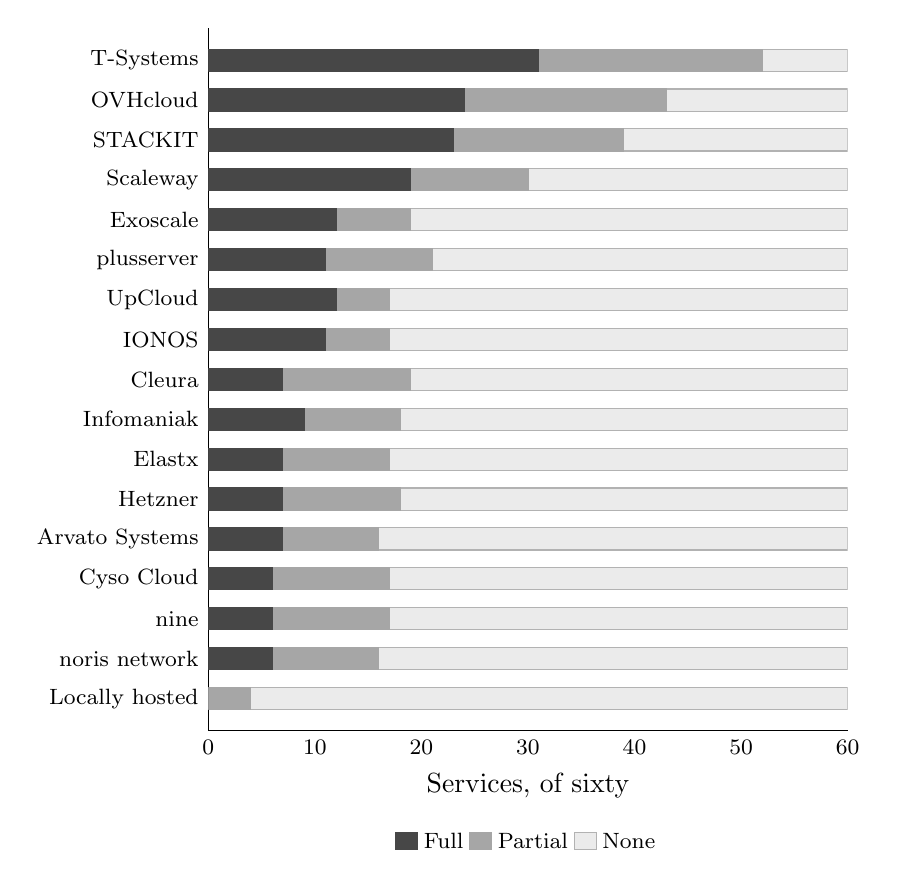
\begin{tikzpicture}
    \begin{axis}[
      xbar stacked,
      width=0.80\textwidth, height=10.5cm,
      xmin=0, xmax=60,
      xlabel={Services, of sixty},
      bar width=8pt,
      enlarge y limits=0.05,
      symbolic y coords={{Locally hosted},{noris network},{nine},{Cyso Cloud},
                         {Arvato Systems},{Hetzner},{Elastx},{Infomaniak},
                         {Cleura},{IONOS},{UpCloud},{plusserver},{Exoscale},
                         {Scaleway},{STACKIT},{OVHcloud},{T-Systems}},
      ytick={{Locally hosted},{noris network},{nine},{Cyso Cloud},
             {Arvato Systems},{Hetzner},{Elastx},{Infomaniak},{Cleura},
             {IONOS},{UpCloud},{plusserver},{Exoscale},{Scaleway},
             {STACKIT},{OVHcloud},{T-Systems}},
      yticklabel style={font=\footnotesize},
      xticklabel style={font=\footnotesize},
      legend style={at={(0.5,-0.13)}, anchor=north, legend columns=3,
                    font=\footnotesize, draw=none},
      tick style={draw=none},
      axis x line*=bottom, axis y line*=left,
    ]
      \addplot[fill=black!72, draw=black!72] coordinates {
        (0,{Locally hosted}) (6,{noris network}) (6,{nine}) (6,{Cyso Cloud})
        (7,{Arvato Systems}) (7,{Hetzner}) (7,{Elastx}) (9,{Infomaniak})
        (7,{Cleura}) (11,{IONOS}) (12,{UpCloud}) (11,{plusserver})
        (12,{Exoscale}) (19,{Scaleway}) (23,{STACKIT}) (24,{OVHcloud})
        (31,{T-Systems})};
      \addplot[fill=black!35, draw=black!35] coordinates {
        (4,{Locally hosted}) (10,{noris network}) (11,{nine}) (11,{Cyso Cloud})
        (9,{Arvato Systems}) (11,{Hetzner}) (10,{Elastx}) (9,{Infomaniak})
        (12,{Cleura}) (6,{IONOS}) (5,{UpCloud}) (10,{plusserver})
        (7,{Exoscale}) (11,{Scaleway}) (16,{STACKIT}) (19,{OVHcloud})
        (21,{T-Systems})};
      \addplot[fill=black!8, draw=black!30] coordinates {
        (56,{Locally hosted}) (44,{noris network}) (43,{nine}) (43,{Cyso Cloud})
        (44,{Arvato Systems}) (42,{Hetzner}) (43,{Elastx}) (42,{Infomaniak})
        (41,{Cleura}) (43,{IONOS}) (43,{UpCloud}) (39,{plusserver})
        (41,{Exoscale}) (30,{Scaleway}) (21,{STACKIT}) (17,{OVHcloud})
        (8,{T-Systems})};
      \legend{Full, Partial, None}
    \end{axis}
  \end{tikzpicture}
  \caption{Verdicts across the sixty reference services, ordered by mean
           coverage.}
  \label{fig:readiness-verdicts}
\end{figure}

The figure separates two groups. Four providers --- T-Systems, OVHcloud, STACKIT
and Scaleway --- cover between a third and a half of the catalogue outright. The
remaining twelve cluster tightly: six to twelve services in full, most of the
rest missing. Locally hosted infrastructure marks the floor, with no managed
equivalent to anything and four partials.

Behind those totals is a service-by-service picture.
\Cref{tab:readiness-services-compare} sets the four leading providers against
the baseline one service at a time, and gives for each service how many of the
seventeen offer a full equivalent.

\footnotesize
\begin{longtable}{@{}p{4.9cm} *{4}{>{\centering\arraybackslash}p{1.75cm}} r@{}}
  \caption{Service-by-service comparison against the \acs{AWS} baseline for
           the four leading providers. Y = a managed equivalent exists in
           full, P = partial, -- = none. The last column counts how many of
           the seventeen offer a full equivalent.}
  \label{tab:readiness-services-compare}\\
  \toprule
  \textbf{\acs{AWS} service} & \textbf{T-Systems} & \textbf{OVHcloud} & \textbf{STACKIT} & \textbf{Scaleway} & \textbf{Full/17} \\
  \midrule
  \endfirsthead
  \toprule
  \textbf{\acs{AWS} service} & \textbf{T-Systems} & \textbf{OVHcloud} & \textbf{STACKIT} & \textbf{Scaleway} & \textbf{Full/17} \\
  \midrule
  \endhead
  \bottomrule
  \endfoot
  \multicolumn{6}{@{}l}{\textit{Web and App Hosting}}\\
  Amplify & P & P & -- & -- & 0 \\
  \midrule
  \multicolumn{6}{@{}l}{\textit{Compute}}\\
  Lambda & Y & P & P & Y & 2 \\
  ECS & Y & Y & Y & Y & 4 \\
  EKS & Y & Y & Y & Y & 10 \\
  EC2 & Y & Y & Y & Y & 16 \\
  Batch & P & P & P & Y & 1 \\
  Elastic Beanstalk & -- & -- & -- & -- & 0 \\
  \midrule
  \multicolumn{6}{@{}l}{\textit{Storage}}\\
  S3 & Y & Y & Y & Y & 16 \\
  S3 Glacier & P & Y & P & P & 1 \\
  EBS & Y & Y & Y & Y & 16 \\
  Backup & Y & Y & Y & P & 5 \\
  EFS & Y & P & -- & -- & 1 \\
  \midrule
  \multicolumn{6}{@{}l}{\textit{Database}}\\
  RDS & Y & Y & Y & Y & 9 \\
  DocumentDB & P & P & -- & P & 0 \\
  DynamoDB & -- & -- & -- & -- & 0 \\
  Timestream & -- & -- & -- & -- & 0 \\
  Aurora & -- & -- & -- & -- & 0 \\
  ElastiCache & Y & Y & Y & P & 5 \\
  Redshift & P & P & P & -- & 0 \\
  \midrule
  \multicolumn{6}{@{}l}{\textit{Networking}}\\
  Application Load Balancer & Y & Y & Y & Y & 9 \\
  Network Load Balancer & Y & Y & Y & P & 4 \\
  VPC & Y & Y & Y & Y & 16 \\
  Route 53 & Y & Y & Y & Y & 10 \\
  API Gateway & Y & P & P & -- & 1 \\
  CloudFront & P & Y & -- & -- & 1 \\
  Direct Connect & Y & Y & Y & -- & 5 \\
  \midrule
  \multicolumn{6}{@{}l}{\textit{AI/ML}}\\
  Rekognition & P & -- & -- & -- & 0 \\
  SageMaker & Y & P & P & P & 1 \\
  Bedrock & -- & -- & -- & -- & 0 \\
  Glue & P & -- & -- & -- & 0 \\
  EMR & P & P & -- & -- & 0 \\
  Athena & P & -- & -- & -- & 0 \\
  \midrule
  \multicolumn{6}{@{}l}{\textit{Security}}\\
  IAM & Y & Y & Y & Y & 14 \\
  Cognito & -- & P & P & -- & 0 \\
  IAM Identity Center & -- & P & P & -- & 0 \\
  KMS & Y & Y & Y & Y & 4 \\
  Secrets Manager & P & P & Y & Y & 2 \\
  Certificate Manager & Y & Y & Y & Y & 4 \\
  GuardDuty & P & P & P & -- & 0 \\
  Security Hub & P & -- & P & -- & 0 \\
  Config & P & -- & P & -- & 0 \\
  Shield & Y & Y & Y & P & 3 \\
  WAF & Y & Y & Y & -- & 3 \\
  CloudTrail & Y & P & Y & P & 2 \\
  \midrule
  \multicolumn{6}{@{}l}{\textit{Monitoring}}\\
  CloudWatch & Y & P & P & P & 1 \\
  SNS & Y & P & P & P & 1 \\
  Systems Manager & P & P & P & -- & 0 \\
  Cost Explorer & Y & Y & Y & Y & 16 \\
  \midrule
  \multicolumn{6}{@{}l}{\textit{Dev/Deploy}}\\
  CodeBuild & P & -- & -- & -- & 0 \\
  CodeDeploy & P & -- & -- & -- & 0 \\
  CodePipeline & P & -- & -- & -- & 0 \\
  ECR & Y & Y & Y & Y & 6 \\
  CloudFormation & Y & P & P & -- & 1 \\
  \midrule
  \multicolumn{6}{@{}l}{\textit{IoT}}\\
  IoT Core & Y & P & -- & P & 1 \\
  IoT Device Management & Y & -- & -- & -- & 1 \\
  \midrule
  \multicolumn{6}{@{}l}{\textit{Messaging}}\\
  SQS & Y & Y & Y & Y & 4 \\
  EventBridge & P & -- & -- & -- & 0 \\
  Step Functions & -- & -- & -- & -- & 0 \\
  SES & P & Y & P & Y & 2 \\
  Kinesis & P & -- & -- & -- & 0 \\
\end{longtable}
\normalsize

\Cref{fig:readiness-ranking} ranks the providers by mean coverage, with the
remaining gap to the baseline shown alongside.

\begin{figure}[htbp]
  \centering
  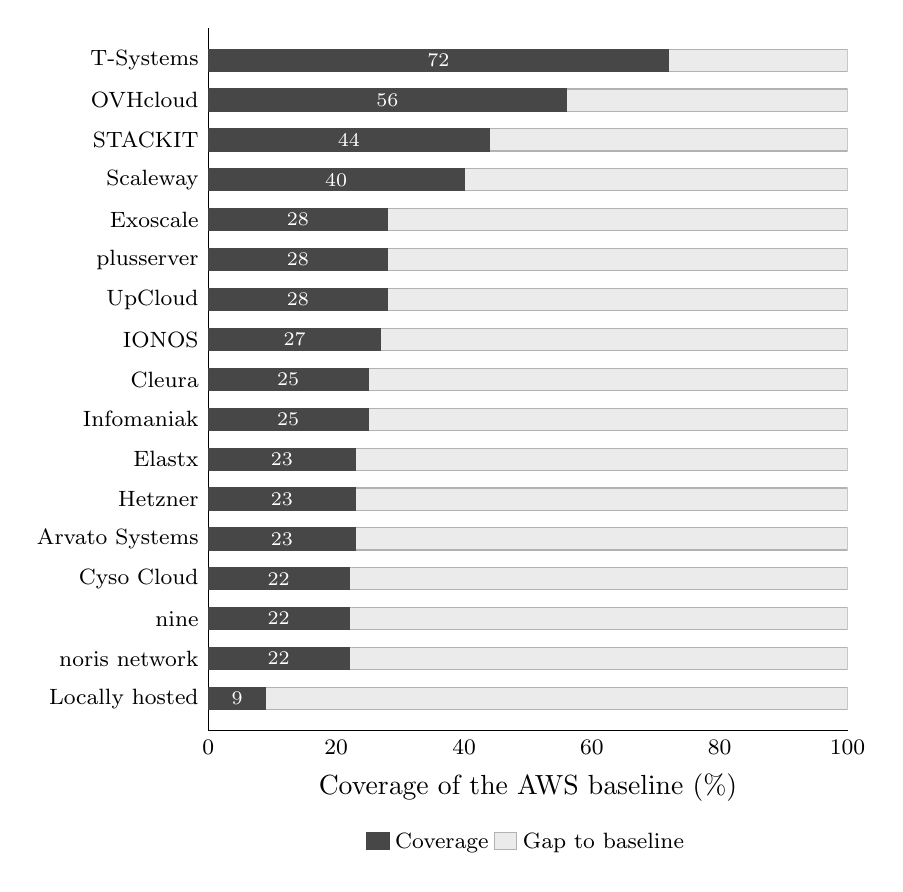
\begin{tikzpicture}
    \begin{axis}[
      xbar stacked,
      width=0.80\textwidth, height=10.5cm,
      xmin=0, xmax=100,
      xlabel={Coverage of the \acs{AWS} baseline (\%)},
      bar width=8pt,
      enlarge y limits=0.05,
      symbolic y coords={{Locally hosted},{noris network},{nine},{Cyso Cloud},
                         {Arvato Systems},{Hetzner},{Elastx},{Infomaniak},
                         {Cleura},{IONOS},{UpCloud},{plusserver},{Exoscale},
                         {Scaleway},{STACKIT},{OVHcloud},{T-Systems}},
      ytick={{Locally hosted},{noris network},{nine},{Cyso Cloud},
             {Arvato Systems},{Hetzner},{Elastx},{Infomaniak},{Cleura},
             {IONOS},{UpCloud},{plusserver},{Exoscale},{Scaleway},
             {STACKIT},{OVHcloud},{T-Systems}},
      yticklabel style={font=\footnotesize},
      xticklabel style={font=\footnotesize},
      legend style={at={(0.5,-0.13)}, anchor=north, legend columns=2,
                    font=\footnotesize, draw=none},
      tick style={draw=none},
      axis x line*=bottom, axis y line*=left,
    ]
      \addplot[fill=black!72, draw=black!72,
               nodes near coords,
               nodes near coords style={font=\scriptsize, text=white}]
        coordinates {
        (9,{Locally hosted}) (22,{noris network}) (22,{nine}) (22,{Cyso Cloud})
        (23,{Arvato Systems}) (23,{Hetzner}) (23,{Elastx}) (25,{Infomaniak})
        (25,{Cleura}) (27,{IONOS}) (28,{UpCloud}) (28,{plusserver})
        (28,{Exoscale}) (40,{Scaleway}) (44,{STACKIT}) (56,{OVHcloud})
        (72,{T-Systems})};
      \addplot[fill=black!8, draw=black!30] coordinates {
        (91,{Locally hosted}) (78,{noris network}) (78,{nine}) (78,{Cyso Cloud})
        (77,{Arvato Systems}) (77,{Hetzner}) (77,{Elastx}) (75,{Infomaniak})
        (75,{Cleura}) (73,{IONOS}) (72,{UpCloud}) (72,{plusserver})
        (72,{Exoscale}) (60,{Scaleway}) (56,{STACKIT}) (44,{OVHcloud})
        (28,{T-Systems})};
      \legend{Coverage, Gap to baseline}
    \end{axis}
  \end{tikzpicture}
  \caption{Mean coverage across the thirteen dimensions, with the remaining gap
           to the \acs{AWS} baseline.}
  \label{fig:readiness-ranking}
\end{figure}

This ranking runs close to the opposite of the sovereignty ranking in
\cref{fig:sov-ranking}. T-Systems Open Telekom Cloud scored lowest of the
eighteen on sovereignty and covers most of the catalogue here. STACKIT scored
highest on sovereignty and comes third. noris network was third on sovereignty
and sixteenth here. The two results are measuring different things, and a
provider that does well on one gives no reason to expect it will do well on the
other --- which is why they are kept apart until \cref{ch:evaluation}.
